\subsection{Intrinsic Randomness of Quantum Measurements}\label{sec:from-wave-particle-duality-to-quantum-states:intrinsic-randomness-of-quantum-measurements}

\begin{flushleft}
    \textcolor{Green3}{\faIcon{question-circle} \textbf{Individual detection events are unpredictable}}
\end{flushleft}
We have already established that electrons exhibit \textbf{wave-like diffraction} but are detected as \textbf{individual, localized particles}. Now we want to investigate a different question: \textbf{\emph{can we predict where the next electron will be detected?}} This question introduces one of the most important features of quantum mechanics: \textbf{randomness in measurement outcomes}.

\highspace
Let's consider the single-electron experiment again (\autopageref{sec:experiment-electron-diffraction}):
\begin{equation*}
    \text{electron gun}
    \rightarrow
    \text{crystal}
    \rightarrow
    \text{fluorescent screen}
\end{equation*}
We send electrons one at a time, keeping the experimental conditions unchanged. In particular, the electrons are prepared with the same nominal energy and momentum, and the crystal and screen remain in the same positions.

\highspace
As we have seen, if we repeat the experiment only a few times (e.g., 3 times), we might observe:
\begin{equation*}
    e_1 \rightarrow x_1, \quad
    e_2 \rightarrow x_2, \quad
    e_3 \rightarrow x_3
\end{equation*}
Where $e_i$ is the $i$-th electron and $x_i$ is the position on the screen where it is detected. Even though we repeat the same preparation procedure, the detection positions $x_1$, $x_2$, and $x_3$ are \textbf{different} and \textbf{unpredictable}. So the important observation was that \hl{the next detection position cannot be determined in advance from the information supplied by the experimental preparation or from the previous detections.}

\highspace
\textcolor{Green3}{\faIcon{question-circle} \textbf{Why was this observation surprising?}} Because a classical particle, like a bullet, would always hit the same spot on the screen if it is prepared in the same way.

\highspace
In classical mechanics, if we know a particle's initial position and momentum, together with the forces acting on it, we can in principle calculate its trajectory:
\begin{equation*}
    \left(x(0),p(0)\right)
    +
    \text{equations of motion}
    \longrightarrow
    x(t)
\end{equation*}
Therefore, we can predict where the particle will arrive. If our classical prediction is inaccurate, we might suspect that we did not know the initial conditions precisely enough.

\highspace
Instead, \hl{quantum mechanics changes this situation.} Even when we prepare an electron in the same quantum state and repeat the same measurement, the standard quantum description generally does not provide a definite position for the next detection. Instead, it provides probabilities for different possible outcomes.

\highspace
At this stage, we do not need to calculate those probabilities. What matters is the experimental observation:
\begin{equation*}
    \text{same preparation procedure}
    \not\Rightarrow
    \text{same detection position}
\end{equation*}
Notice that this does \textbf{not} mean quantum mechanics cannot predict anything. It means that \textbf{predicting the individual result} and \textbf{predicting the statistics of many results} are \hl{different tasks}.

\highspace
\textcolor{Green3}{\faIcon{question-circle} \textbf{Does unpredictable mean equally likely everywhere?}} No. Suppose the fluorescent screen has three possible detection regions: $A$, $B$, and $C$. The electron might arrive in any of them, but it does not follow that
\begin{equation*}
    P(A)=P(B)=P(C)
\end{equation*}
Some regions may be much more likely than others, and some may have a negligible probability of detection. That is perfectly compatible with the diffraction pattern we observed in the previous section.
\begin{equation*}
    \text{unpredictable individual outcome}\neq\text{uniformly random outcome}
\end{equation*}

\highspace
\textcolor{Green3}{\faIcon{question-circle} \textbf{Have we already demonstrated intrinsic randomness?}}
\footnote{\textbf{Intrinsic} means inherent to the nature of something, rather than caused by external factors. In quantum physics, \emph{intrinsic randomness} refers to randomness that is fundamental to the measurement outcome, not merely due to incomplete knowledge or imperfect measuring instruments.} We should distinguish the observation from its interpretation:
\begin{itemize}
    \item What we have observed is that individual detection positions are unpredictable under our controlled experimental conditions.
    \item That \hl{observation alone does not prove that randomness is fundamentally intrinsic rather than a consequence of unknown variables.}
\end{itemize}
One might still ask whether some inaccessible information determines each outcome, just as an apparently random coin toss can be determined by its initial conditions. We will not answer it yet, but we will investigate it in the next pages.

\highspace
Now, we have identified the randomness of individual detections. The next question is: \emph{\textbf{if individual outcomes are unpredictable, how can the diffraction pattern be so reproducible?}}

\highspace
\begin{takeawaysbox}
    \begin{equation*}
        \begin{gathered}
            \text{One electron is sent toward the crystal.}\\
            \Downarrow\\
            \text{One localized detection occurs.}\\
            \Downarrow\\
            \text{Its position cannot generally be predicted in advance.}
        \end{gathered}
    \end{equation*}
    Quantum measurements can produce different individual outcomes even when the system is prepared in the same way.
\end{takeawaysbox}

\newpage

\begin{flushleft}
    \textcolor{Green3}{\faIcon{chart-bar} \textbf{Statistical regularity from many repetitions}}
\end{flushleft}
Thus \hl{we cannot predict where the next electron will be detected}, but this raises an apparent contradiction: if individual electron detections are unpredictable, \textbf{\emph{how can the diffraction pattern be so regular and reproducible?}} In other words, how can we reconcile the unpredictability of individual events with the predictability of the overall pattern?

\highspace
\textcolor{Green3}{\faIcon{random} \textbf{Random individual events do not imply a random overall distribution.}} Let's return to our electron-diffraction experiment. We prepare the electron gun, crystal and fluorescent screen, and send electrons \textbf{one at a time}. For each electron, we observe one localized flash at a position that we cannot predict beforehand.

\highspace
Now suppose we repeat the experiment $N$ times, without changing the experimental conditions. We observe:
\begin{equation*}
    x_1, x_2, x_3, \ldots, x_N
\end{equation*}
Where $x_i$ is the detection position of electron $i$. At first, with only a few electrons, the spots appear scattered without an obvious pattern. However, as the number of detections increases, something remarkable happens: \hl{the detections accumulate preferentially in certain regions, reproducing the characteristic diffraction pattern.}

\highspace
This is the same experimental picture developed earlier on \autopageref{fig:single-electron-detection-accumulation}, where individual localized flashes appear at unpredictable positions, but they occur with a spatial distribution associated with diffraction.

\begin{figure}[htbp]
    \centering
    \tikzcachefilename{electron-diffraction-accumulation}

    \begin{tikzpicture}[
            font=\small,
            screen/.style={
                draw=black!60,
                fill=gray!4,
                rounded corners=2pt,
                line width=0.75pt
            },
            detection/.style={
                fill=blue!75!black,
                opacity=0.78
            }
        ]

        % Three accumulation stages.
        %
        % Each screen has the same underlying
        % probability distribution.
        %
        % The random seed is reset for every panel:
        % the first N detections are preserved as
        % further detections accumulate.

        \foreach \sx/\N/\stage in {
            0/15/{Few detections},
            4.25/120/{Emerging pattern},
            8.5/700/{Established pattern}
        }{

            \begin{scope}[xshift=\sx cm]

                % Panel heading
                \node[
                    font=\small\bfseries,
                    align=center
                ] at (0,2.25) {\stage};

                % Fluorescent screen
                \draw[screen]
                (-1.78,-1.78)
                rectangle (1.78,1.78);

                % Reproducible random sequence
                \pgfmathsetseed{2026}

                \foreach \k in {1,...,\N}{

                    % Choose a diffraction maximum.
                    %
                    % Illustrative 3x3 arrangement:
                    % the central maximum has the
                    % largest statistical weight.
                    %
                    % Probabilities are generated by
                    % independently sampling the two
                    % coordinate directions.

                    \pgfmathsetmacro{\rx}{rnd}
                    \pgfmathsetmacro{\ry}{rnd}

                    \pgfmathsetmacro{\cx}{
                        ifthenelse(
                            \rx < 0.19,
                            -1.05,
                            ifthenelse(
                                \rx < 0.81,
                                0,
                                1.05
                            )
                        )
                    }

                    \pgfmathsetmacro{\cy}{
                        ifthenelse(
                            \ry < 0.19,
                            -1.05,
                            ifthenelse(
                                \ry < 0.81,
                                0,
                                1.05
                            )
                        )
                    }

                    % Random displacement around
                    % the selected maximum.
                    %
                    % Sum of uniform variables gives
                    % a roughly bell-shaped spread.

                    \pgfmathsetmacro{\dx}{
                        0.25*(rnd+rnd+rnd+rnd-2)
                    }

                    \pgfmathsetmacro{\dy}{
                        0.25*(rnd+rnd+rnd+rnd-2)
                    }

                    % One electron produces one
                    % localized detection event.

                    \fill[detection]
                    ({\cx+\dx},{\cy+\dy})
                    circle[radius=0.026];
                }

                % Number of detections
                \node[
                    font=\small,
                    text=black!70
                ] at (0,-2.12)
                {$N=\N$};

            \end{scope}
        }

        % Direction of accumulation
        \draw[
            -{Latex[length=2.5mm]},
            line width=0.9pt,
            black!65
        ]
        (-1.4,-2.75) -- (9.9,-2.75);

        \node[
            fill=white,
            inner sep=3pt,
            font=\small,
            text=black!75
        ] at (4.25,-2.75)
        {Increasing number of detections};

    \end{tikzpicture}
\end{figure}

\noindent
So we must distinguish between two different types of predictions:
\begin{itemize}
    \item \textbf{Individual prediction}: \emph{where will the next electron arrive?}
    \item \textbf{Statistical prediction}: \emph{how frequently will electrons arrive in different regions after many repetitions?}
\end{itemize}
Quantum mechanics answers these questions differently.

\highspace
\textcolor{Green3}{\faIcon{chart-bar} \textbf{From individual positions to relative frequencies.}} Imagine dividing the fluorescent screen into regions $A$, $B$, and $C$. After sending $N$ electrons, we count how many were detected in each region: $N_A$, $N_B$, and $N_C$. If these are all the possible detection regions, then:
\begin{equation*}
    N_A+N_B+N_C=N
\end{equation*}
We can define the \textbf{relative frequency} of detections in region $A$:
\begin{equation*}
    f_A(N)=\frac{N_A}{N}
\end{equation*}
For example, imagine that after 1,000 detected electrons we have:
\begin{center}
    \begin{tabular}{@{} c c c @{}}
        \toprule
        Region & Detections & Relative Frequency \\
        \midrule
        $A$ & 700 & 70\% \\
        $B$ & 250 & 25\% \\
        $C$ & 50 & 5\% \\
        \bottomrule
    \end{tabular}
\end{center}

\begin{figure}[!htbp]
    \centering

    \definecolor{qBlue}{RGB}{40,92,190}
    \definecolor{qTeal}{RGB}{20,140,135}
    \definecolor{qOrange}{RGB}{220,125,35}

    \tikzsetnextfilename{relative-frequency-screen-regions}

    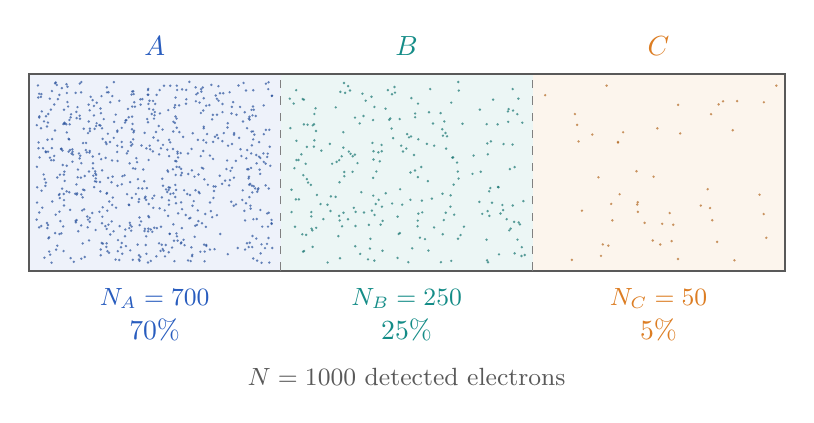
\begin{tikzpicture}[font=\small]

        % Three equal-sized screen regions
        \fill[qBlue!8]
        (0,1.0) rectangle (3.2,3.5);

        \fill[qTeal!8]
        (3.2,1.0) rectangle (6.4,3.5);

        \fill[qOrange!8]
        (6.4,1.0) rectangle (9.6,3.5);

        % Region labels
        \node[text=qBlue, font=\bfseries]
        at (1.6,3.85) {$A$};

        \node[text=qTeal, font=\bfseries]
        at (4.8,3.85) {$B$};

        \node[text=qOrange, font=\bfseries]
        at (8.0,3.85) {$C$};

        % Generate 1000 localized detections:
        % 700 in A, 250 in B, 50 in C.
        \pgfmathsetseed{2026}

        \foreach \xstart/\num/\dotcolor in {0/700/qBlue,3.2/250/qTeal,6.4/50/qOrange}{%
            \foreach \i in {1,...,\num}{%

                \pgfmathsetmacro{\xx}{
                    \xstart + 0.10 + 3.00*rnd
                }

                \pgfmathsetmacro{\yy}{
                    1.10 + 2.30*rnd
                }

                \fill[
                    \dotcolor!80!black,
                    opacity=0.68
                ]
                (\xx,\yy)
                circle[radius=0.017];
            }
        }

        % Screen outline
        \draw[black!65, line width=0.7pt]
        (0,1.0) rectangle (9.6,3.5);

        % Region boundaries
        \draw[dashed,black!50]
        (3.2,1.0) -- (3.2,3.5);

        \draw[dashed,black!50]
        (6.4,1.0) -- (6.4,3.5);

        % Detection counts
        \node[text=qBlue]
        at (1.6,0.65) {$N_A=700$};

        \node[text=qTeal]
        at (4.8,0.65) {$N_B=250$};

        \node[text=qOrange]
        at (8.0,0.65) {$N_C=50$};

        % Relative frequencies
        \node[text=qBlue, font=\bfseries]
        at (1.6,0.25) {$70\%$};

        \node[text=qTeal, font=\bfseries]
        at (4.8,0.25) {$25\%$};

        \node[text=qOrange, font=\bfseries]
        at (8.0,0.25) {$5\%$};

        % Total detections
        \node[text=black!65]
        at (4.8,-0.35)
        {$N=1000$ detected electrons};

    \end{tikzpicture}

    \caption{
        \textbf{Relative frequencies of electron detections.}
        A fluorescent screen is divided into three
        equal-sized regions $A$, $B$, and $C$.
        After $N=1000$ detections, the hypothetical
        counts are $N_A=700$, $N_B=250$, and
        $N_C=50$, corresponding to relative
        frequencies of $70\%$, $25\%$, and $5\%$.
        Each dot represents one localized electron
        detection. All values are illustrative.
    }

    \label{fig:relative-frequency-screen-regions}

\end{figure}

\noindent
The \textbf{next electron remains unpredictable}, it might arrive in $A$, $B$, or $C$. But if we repeat the same experiment a sufficiently large number of times, the relative frequencies tend to stabilize near characteristic values. For region $A$:
\begin{equation*}
    f_A(N)\longrightarrow P(A)\quad\text{as }N\rightarrow\infty
\end{equation*}
Under repeated, identically prepared independent trials, $P(A)$ is the probability of obtaining a detection in region $A$. This does \textbf{not} mean that every group of 100 electrons must contain exactly 70 detections in $A$. The counts still fluctuate (see \autoref{fig:relative-frequency-statistical-convergence}, \autopageref{fig:relative-frequency-statistical-convergence}).

\highspace
It means that, as the number of \hl{repetitions becomes large}, the \hl{relative fluctuations become less significant} and the estimated \hl{probabilities become increasingly reliable}. This is what we mean by \definition{Statistical Regularity}.

\newpage

\begin{figure}[!htbp]
    \centering
    \definecolor{qBlue}{RGB}{40,92,190}
    \tikzsetnextfilename{relative-frequency-statistical-convergence}
    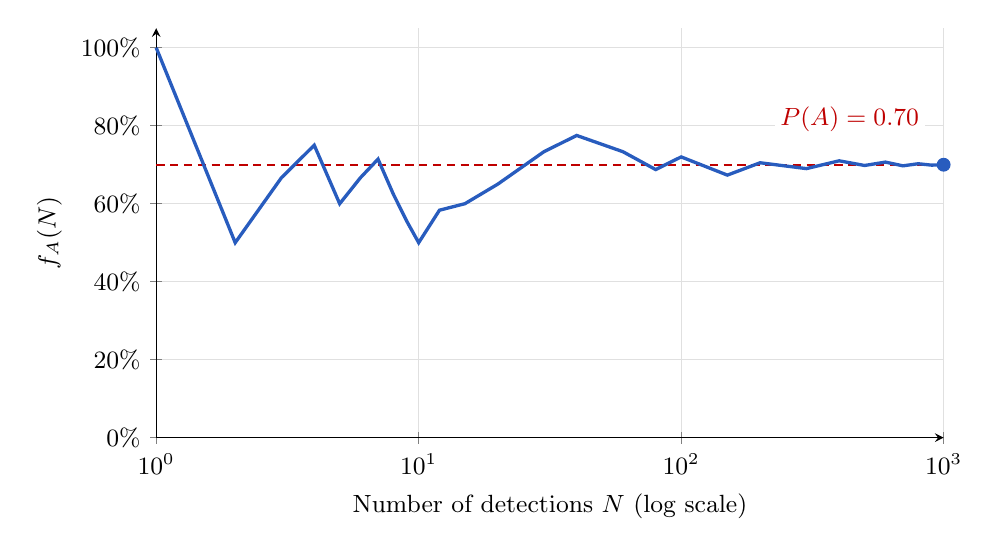
\begin{tikzpicture}

        \begin{axis}[
                width=10.0cm,
                height=5.2cm,
                scale only axis,
                xmode=log,
                log basis x=10,
                xmin=1,
                xmax=1000,
                ymin=0,
                ymax=1.05,
                xtick={1,10,100,1000},
                ytick={0,0.2,0.4,0.6,0.8,1},
                yticklabels={
                    $0\%$,
                    $20\%$,
                    $40\%$,
                    $60\%$,
                    $80\%$,
                    $100\%$
                },
                xlabel={Number of detections $N$ (log scale)},
                ylabel={$f_A(N)$},
                tick label style={font=\small},
                label style={font=\small},
                axis lines=left,
                grid=major,
                grid style={black!12},
                clip=false
            ]

            % Hypothetical probability P(A) = 0.70
            \addplot[
                color=red!75!black,
                densely dashed,
                thick,
                domain=1:1000,
                samples=2
            ] {0.70};

            \node[
                anchor=south east,
                text=red!75!black,
                font=\small,
                fill=white,
                inner sep=2pt
            ] at (axis cs:850,0.77)
            {$P(A)=0.70$};

            % Cumulative relative frequency
            % f_A(N) = N_A / N
            %
            % n    = total detected electrons
            % hits = detections in region A
            %
            % Illustrative cumulative counts.

            \addplot[
                color=qBlue,
                very thick,
                mark=none
            ]
            table[
                x=n,
                y expr=\thisrow{hits}/\thisrow{n}
            ] {
                n    hits
                1    1
                2    1
                3    2
                4    3
                5    3
                6    4
                7    5
                8    5
                9    5
                10   5
                12   7
                15   9
                20   13
                30   22
                40   31
                60   44
                80   55
                100  72
                150  101
                200  141
                300  207
                400  284
                500  349
                600  424
                700  488
                800  562
                900  629
                1000 700
            };

            % Final observed relative frequency
            \addplot[
                only marks,
                mark=*,
                mark size=2.3pt,
                color=qBlue
            ] coordinates {
                (1000,0.70)
            };

        \end{axis}

    \end{tikzpicture}

    \caption{
        \textbf{Statistical convergence of relative frequencies.}
        The cumulative relative frequency
        $f_A(N)=N_A/N$ fluctuates as electrons
        are detected, but tends to stabilize
        near the hypothetical probability
        $P(A)=0.70$ as $N$ increases.
        The logarithmic horizontal axis
        emphasizes the fluctuations at small
        sample sizes. The blue curve connects
        selected cumulative frequencies,
        while the dashed red line represents
        the underlying probability.
        All values are illustrative.
    }
    \label{fig:relative-frequency-statistical-convergence}
\end{figure}

\highspace
\textcolor{Green3}{\faIcon{bullseye} \textbf{How does this explain the diffraction pattern?}} A diffraction pattern contains bright and dark regions. On \autopageref{fig:diffraction-pattern} we saw that, for classical light, brightness is connected to intensity. So now we can give an \hl{experimental interpretation to the electron-diffraction pattern:}
\begin{itemize}
    \item At a position where the electron signal is strong, we observe many detections over time.
        \begin{equation*}
            \text{\textbf{bright} diffraction region} \implies \text{\textbf{high} detection \textbf{frequency}}
        \end{equation*}
    \item At a position where the signal is weak, we observe fewer detections.
        \begin{equation*}
            \text{\textbf{dark} diffraction region} \implies \text{\textbf{low} detection \textbf{frequency}}
        \end{equation*}
\end{itemize}
For an ideal detector, the number of electrons detected per unit area and time gives the local electron arrival flux.
Thus, the \hl{diffraction pattern tells us where electron detections are more or less likely.}
The pattern is not visible because each electron deposits a fraction of itself in every bright region.
It emerges because many complete, individually detected electrons accumulate with different frequencies in different regions.
\begin{equation*}
    \text{One electron} \rightarrow \text{one localized detection}
\end{equation*}
\begin{equation*}
    \text{Many repetitions} \rightarrow \text{reproducible spatial distribution}
\end{equation*}

\newpage

\noindent
\textcolor{Green3}{\faIcon{chart-area} \textbf{What does quantum mechanics predict?}} In classical mechanics, we often try to predict the trajectory of each particle, given sufficiently precise initial conditions.

\highspace
\hl{In quantum mechanics, the standard theory generally predicts \textbf{probabilities for measurement outcomes}.}
For example, instead of determining the exact position $x$ at which the next electron will be detected, the theory can predict a probability distribution over possible positions.

\highspace
Those probabilities can then be tested experimentally by repeating the preparation and measurement many times.
Later, we will learn the \hl{mathematical rule that connects quantum states with measurement probabilities:} the \textbf{Born rule}.
For now, we do not need that rule. The experimental observation already tells us that our model must explain both unpredictable individual detections and reproducible statistical distributions.

\highspace
\textcolor{Green3}{\faIcon{balance-scale} \textbf{Randomness and regularity are compatible.}} A random process can follow a well-defined probability distribution. So, \hl{randomness describes the uncertainty of individual outcomes}, while \hl{statistical regularity describes the reproducibility of their distribution.}
\begin{center}
    \resizebox{\textwidth}{!}{%
        \begin{tabular}{@{} l | l @{}}
            \toprule
            \textbf{Individual measurement} & \textbf{Many repeated measurements} \\
            \midrule
            \hl{One} localized flash & A \hl{collection} of localized flashes \\
            Exact position \hl{unpredictable} & Relative frequencies become \hl{stable} \\
            Different outcomes are possible & The overall diffraction pattern is \hl{reproducible} \\
            \hl{Random} individual result & \hl{Predictable} statistical distribution \\
            \bottomrule
        \end{tabular}%
    }
\end{center}

\highspace
\begin{takeawaysbox}
    \begin{equation*}
        \begin{gathered}
            \text{Individual electron detections are unpredictable}\\
            \Downarrow\\
            \text{Repeat the experiment many times}\\
            \Downarrow\\
            \text{Relative detection frequencies stabilize}\\
            \Downarrow\\
            \text{A reproducible diffraction pattern emerges}
        \end{gathered}
    \end{equation*}
    Quantum Mechanics does not need to predict each individual detection to make precise experimental predictions. It must correctly predict the statistical distribution of possible outcomes.
\end{takeawaysbox}

\newpage

\begin{flushleft}
    \textcolor{Green3}{\faIcon{question-circle} \textbf{Why the diffraction pattern is not caused by interactions between particles}}
\end{flushleft}
We have already encountered this topic on \autopageref{sec:single-particle-regime}, so this part is mainly about understanding \textbf{\emph{why the single-particle experiment is such an important experimental test}}.

\highspace
Our initial observation was that \hl{an electron beam produces a diffraction pattern.} We interpreted this as evidence of wave-like behaviour. But there is a possible objection: \emph{\textbf{what if the diffraction pattern is caused by interactions between electrons rather than by the wave-like nature of electrons?}}

\highspace
This is not an unreasonable hypothesis. Electrons have negative electric charge. Consequently, they exert repulsive electric forces on one another. If many electrons travel through the apparatus\footnote{%
    The apparatus is the complete experimental setup used to perform electron diffraction: the electron gun, the crystal, and the fluorescent screen. The electron gun emits electrons, the crystal scatters them, and the fluorescent screen detects their arrival (see \autopageref{fig:single-particle-regime}).%
} simultaneously, they may influence each other's motion. One could therefore \hl{hypothesize that their collective interactions produce the observed spatial distribution.} Thus, the question becomes: \emph{\textbf{how can we test this hypothesis experimentally?}}

\highspace
\textcolor{Green3}{\faIcon{trash-alt} \textbf{Eliminate electron-electron interactions.}} We change a simple experimental parameter: the \textbf{electron emission rate}. We reduce the beam current until successive electrons are sufficiently separated in time that only one incident electron is inside the apparatus at any given moment.

\highspace
Mathematically, if $t_f$ is the \hl{time needed for an electron to travel through the apparatus}, we want the interval between emissions to satisfy approximately: $\Delta t\gg t_f$.

\begin{figure}[!htp]
    \centering
    \tikzsetnextfilename{flight-windows}
    \begin{tikzpicture}[
            x=0.93cm, y=1cm,
            >=Stealth,
            every node/.style={font=\small},
            win/.style={draw=blue!70!black, fill=blue!15, rounded corners=1pt}
        ]

        %% ===================== (a) high rate =====================
        \node[anchor=west] at (0,2.2) {\textbf{(a)} high rate: $\Delta t \lesssim t_f$};
        \foreach \i in {0,...,14}{
            \pgfmathsetmacro{\x}{0.7*\i}
            \pgfmathsetmacro{\y}{0.45*mod(\i,3)}
            \draw[win] (\x,\y) rectangle ++(1.8,0.35);
        }
        \draw[->] (-0.1,-0.3) -- (12,-0.3) node[right] {$t$};
        \draw[dashed, thick, orange!80!black] (1.5,-0.5) -- (1.5,1.5);
        \node[orange!80!black, anchor=north west, align=left] at (0,-0.55)
        {3 electrons inside at once: possible interaction};

        %% ===================== (b) low rate =====================
        \begin{scope}[shift={(0,-3.9)}]
            \node[anchor=west] at (0,2.2) {\textbf{(b)} low rate: $\Delta t \gg t_f$};
            \foreach \k/\x in {1/0.2, 2/5, 3/9.8}{
                \draw[win] (\x,0) rectangle ++(1.8,0.35);
                \node[anchor=west, inner sep=2pt] at (\x+0.05,0.175) {\footnotesize $e_\k$};
                \draw[dotted, gray!60!black] (\x,0.35) -- (\x,1.0);
            }
            \draw[->] (-0.1,-0.3) -- (12,-0.3) node[right] {$t$};
            \draw[<->, gray!60!black] (0.2,0.85) -- (5,0.85) node[midway, above] {$\Delta t$};
            \draw[<->, gray!60!black] (5,0.85) -- (9.8,0.85) node[midway, above] {$\Delta t$};
            \draw[dashed, thick, green!50!black] (6.3,-0.5) -- (6.3,0.6);
            \node[green!50!black, anchor=north, align=center] at (6.3,-0.55)
            {only 1 electron inside:\\ no $e^-\!\leftrightarrow e^-$ interaction};
        \end{scope}
    \end{tikzpicture}
\end{figure}

\noindent
Now electron $e_1$ has completed its journey before electron $e_2$ enters the apparatus.
Therefore, the two incident electrons \textbf{cannot interact} with one another during their passage.

\highspace
\textcolor{Green3}{\faIcon{question-circle} \textbf{What happens experimentally?}} We already know the answer:
\begin{itemize}
    \item First, each electron produces one localized flash on the fluorescent screen.
    \item Then, after repeating the experiment many times, the accumulated detections reproduce the diffraction pattern.
\end{itemize}
This result is decisive for our hypothesis, because if the diffraction pattern required interactions \textbf{between incident electrons}, it should disappear when those interactions are eliminated. But it does \textbf{not disappear}. Therefore, \hl{electron-electron interactions are not necessary for diffraction.}

\highspace
\textcolor{Green3}{\faIcon{question-circle} \textbf{Does this mean the electron does not interact with anything?}} No! We have eliminated interactions \textbf{between different incident electrons}, but the incident electron still interacts with the crystal. The \hl{electron is scattered by the periodic structure of the crystal.} Without the scattering structure, this particular diffraction experiment would \textbf{not produce the same pattern}.
\begin{equation*}
    \underbrace{\text{electron}\leftrightarrow\text{electron}}_{\text{excluded by the experiment}}
    \qquad
    \underbrace{\text{electron}\leftrightarrow\text{crystal}}_{\text{still present (and necessary?)}}
\end{equation*}

\begin{takeawaysbox}
    \begin{equation*}
        \begin{gathered}
            \text{Hypothesis: diffraction is caused by}\\
            \text{interactions among incident electrons}\\
            \Downarrow\\
            \text{Send one electron at a time}\\
            \Downarrow\\
            \text{Electron-electron interactions are eliminated}\\
            \Downarrow\\
            \text{The diffraction pattern still emerges}\\
            \Downarrow\\
            \text{The hypothesis is rejected}
        \end{gathered}
    \end{equation*}
    Wave-like diffraction is not a collective effect produced by interactions among the incident electrons. It is a feature that our description of individual electrons must accommodate (i.e., \emph{must be capable of explaining the phenomenon}), or in other words, our mathematical model of a single electron must be able to explain why repeated single-electron experiments produce a diffraction pattern.

    \highspace
    In summary, we \hl{need a theory describing even a single electron must contain the ingredients necessary to predict the diffraction pattern.}
\end{takeawaysbox}